\chapter{Results}
\section{Babel Stream}
\begin{figure}[h]
  \center
  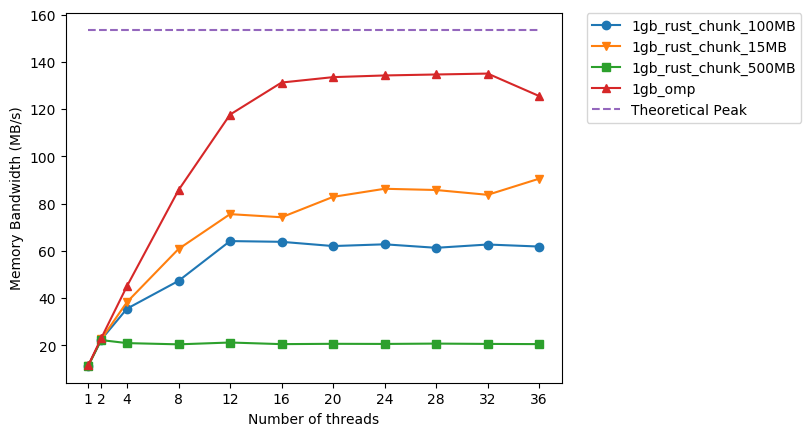
\includegraphics[width=.8\linewidth]{figs/babel/Dot.png}
  \caption{Babel Stream: Dot product bandwidth}
  \label{fig:babel-dot}
\end{figure}
Babel stream results show that Rayon is unable to scale as well as OpenMP. This is likely because of the CC-Numa layout of the system, and Rayon's affinity schedule. I might include a diagram here to show exactly what I mean. Is it worth getting the legend outside the box? would make things look neater

I might generate this figure again but without the 500MB rust run, and include chunkless para init runs instead on add, triad etc
\section{Sparse Matrix}
\section{K-means}
\section{Questionnaire}
